%Plantilla para proyectos modulares de ciencias básicas.
%Para usar en los proyectos de Lic. en Física. Para otras carreras consulte a su coordinador.
%
%Edite donde se indica y sea necesario.
%
%Versión 2.0
%


\documentclass[letterpaper,12pt]{article}
\usepackage[utf8]{inputenc}
\usepackage[table]{xcolor}
\usepackage{graphicx}
\usepackage{epsfig}
\usepackage{float}
\usepackage[hidelinks]{hyperref}
\usepackage{array}
\usepackage{lastpage}
\usepackage[spanish,es-tabla]{babel} % Se considera TABLA en lugar de CUADRO en las tablas. Modificado por Rotosca
\usepackage{fancyhdr}
\usepackage{geometry}

%Matemática
\usepackage{amsmath}
\usepackage{amsfonts}
\usepackage{amssymb}
\usepackage{tabularx}
\usepackage{multicol}
\usepackage{soul}
\usepackage{amstext}


%tamaño de la fuente en las secciones.
\usepackage{sectsty}
\sectionfont{\fontsize{12}{15}\selectfont}
\subsectionfont{\fontsize{11}{15}\selectfont}


\definecolor{AzulModular}{cmyk}{1.0,0.49,0.0,0.47}%color #4365A4

\setlength{\parindent}{0.95cm}

\geometry{
  left=0.748in,
  right=0.780in,
  top=3.9cm,
  headheight=1.9cm,
  headsep=0.5cm,
%  bottom=3.54cm,
  footskip=2.54cm,
}

\decimalpoint

\graphicspath{{figuras/}}

\newcommand{\cfbox}[2]{%
    \colorlet{currentcolor}{.}%
    {\color{#1}%
    \fbox{\color{currentcolor}#2}}%
}


\pagestyle{fancy}
\cfoot{}
\renewcommand{\headrulewidth}{0pt}
\fancyhead[CO,LO,RO]{} %% clear out all headers
\fancyhead[C]{%
          \begin{tabular}{m{1.5cm}m{11.5cm}m{2.5cm}}
          
\includegraphics[height=1.5cm]{udg_4365A4} &\cellcolor{AzulModular}
          \centering
          \cfbox{white}{%
            \begin{minipage}{10.5cm}
              \centering
              \textcolor{white}{Evaluación Modular, Departamento de Física, 2026B}
            \end{minipage}
            }
            &
          \centering
          \tiny{Licenciatura en Física\\%para usar en otras carreras consulte a su coordinador
%%%%%%%%%%%%%%%%%%%%%%%%%%%%%%%%%%%%%%%%%%%%%%%%%%%%%%%%%%%%%%%%%%%%%%%%%%%%%%%%%%%%%%%%%%%%%%%%%
            Modular: [I, II o III]\\ %elija el que corresponda ejemplo :  Modular : I
%%%%%%%%%%%%%%%%%%%%%%%%%%%%%%%%%%%%%%%%%%%%%%%%%%%%%%%%%%%%%%%%%%%%%%%%%%%%%%%%%%%%%%%%%%%%%%%%%
            Página \thepage \hspace{1pt} de \pageref{LastPage}\\
          }\tabularnewline
%          \hline
          \end{tabular}%
}

%%%%%%%%%%%%%%%%%%%%%%%%%%%%%%%%%%%%%%%%%%%%%%%%%%%%%%%%%%%%%%%%%%%%%%%%%%%%%%%%%%%%%%%%%%%%%%%%%
\title{\fontsize{0.5cm}{0.5cm}\selectfont
\textit{\textbf{Discriminación entre explosiones nucleares subterráneas y sismos naturales mediante $m_b$ y $M_s$ calculadas desde sismogramas: reproducción, validación física y prueba con eventos de magnitud equiparable}}
}
\author{ \fontsize{0.35cm}{0.5cm}\selectfont
\textit{Luis Alberto Román Verde$^1$} \\
        \and \fontsize{0.35cm}{0.5cm}\selectfont \textit{\textbf{Asesor:} [Nombre del asesor]$^1$}
	}

\date{\small
  $^1$\fontsize{0.35cm}{0.5cm}\selectfont \textit{luis.roman4456@alumnos.udg.mx\\ Departamento de Física, CUCEI, Universidad de Guadalajara\\
    Blvd. Marcelino García Barragán 1421, Col. Olímpica, Guadalajara Jal., C. P. 44430, México}\\[2ex]
  }
%%%%%%%%%%%%%%%%%%%%%%%%%%%%%%%%%%%%%%%%%%%%%%%%%%%%%%%%%%%%%%%%%%%%%%%%%%%%%%%%%%%%%%%%%%%%%%%%%

%%%%%%%%%%%%%%%%%%%%%%%%%%%%%%% Comienza el documento%%%%%%%%%%%%%%%%%%%%%%%%%%%%%%%%%%5
\begin{document}
\maketitle
\thispagestyle{fancy}

\section*{Resumen}
Se estudia el discriminante sísmico $D=m_b-M_s$, que separa explosiones nucleares subterráneas de sismos naturales porque una fuente explosiva, compacta y breve, radía proporcionalmente más energía a periodos de $\sim$1~s (ondas P) que a $\sim$20~s (ondas Rayleigh). Se reprodujo un análisis de 20 explosiones y 20 sismos de 1990--1991 en el que ambas magnitudes se calculan desde sismogramas crudos (retiro de la respuesta instrumental, simulación WWSSN y fórmulas IASPEI), sin usar magnitudes de catálogo. Se verificaron las 1142 lecturas por estación y las métricas publicadas: umbral $D\geq0.3185$ y 95\% de aciertos con validación cruzada dejando un evento fuera. Sin embargo, se encontró que la cohorte está sesgada por tamaño: $M_s$ por sí sola clasifica los 40 eventos. Para aislar el efecto físico se compararon pares de igual $m_b$: Lop~Nor (1990) contra Taiwán (1990), y un par nuevo descargado y procesado con el mismo código, la prueba de Corea del Norte del 9-sep-2016 contra el sismo de Gyeongju del 12-sep-2016. En ambos, a igual $m_b$, la explosión presenta $M_s$ menor (por 2.0 y 0.77 unidades) y $D$ mayor en 8/8 y 18/19 estaciones comunes. No obstante, el sismo de Gyeongju ($D=0.35$) cae del lado ``explosión'' del umbral fijo, lo que muestra que la frontera debe depender de $m_b$.

\section*{Introducción}
La verificación del Tratado de Prohibición Completa de los Ensayos Nucleares requiere distinguir, a partir de registros sísmicos, si una fuente es una explosión o un sismo tectónico \cite{bowers}. Uno de los criterios más antiguos y robustos compara dos magnitudes medidas en bandas de frecuencia distintas: la magnitud de ondas de cuerpo $m_b$, obtenida de ondas P de periodo $\sim$1~s, y la magnitud de ondas superficiales $M_s$, obtenida de ondas Rayleigh de periodo $\sim$20~s.

La base física es la diferencia en el espectro de la fuente \cite{stevens}. Una explosión subterránea es una fuente casi isótropa, de dimensión reducida y duración de fracciones de segundo; su frecuencia de esquina es alta y su espectro es relativamente plano hasta frecuencias de $\sim$1~Hz. Un sismo es una dislocación de cizalla que se propaga sobre una falla de kilómetros durante varios segundos; para un mismo nivel de ondas P de 1~s, su espectro contiene mucha más energía a 20~s. En consecuencia, a igual $m_b$ una explosión tiene $M_s$ menor, es decir, $D=m_b-M_s$ mayor.

El objetivo de este trabajo fue (i) explicar y reproducir un análisis reciente que calcula $m_b$ y $M_s$ ``desde cero'' para 40 eventos de la Guerra Fría tardía, (ii) evaluar críticamente su validez física y estadística, y (iii) probar el discriminante en la situación que realmente importa: eventos de magnitud equiparable.

\section*{Metodología}

\subsection*{Datos y corrección instrumental}
Para cada evento se tomaron del catálogo únicamente la hora de origen, el hipocentro y el tipo de fuente. Se solicitaron hasta 60 canales verticales BHZ entre $20^\circ$ y $160^\circ$ de distancia epicentral a los servicios FDSN de EarthScope (formas de onda MiniSEED y respuestas StationXML). A cada traza se le retiró la media y la tendencia, se le aplicó un taper de 2\% y se deconvolucionó la respuesta instrumental hasta desplazamiento del suelo con ObsPy \cite{obspy}. Después se convolucionó con las respuestas de los sismógrafos WWSSN de periodo corto (SP) y largo (LP) \cite{iaspei}, para los que están calibradas las fórmulas de magnitud.

\subsection*{Magnitudes IASPEI}
En la traza WWSSN-SP se busca, entre la llegada teórica de P (modelo IASP91 \cite{iasp91}) y 5~s antes de PP, el ciclo de mayor amplitud con periodo $T<3$~s. La amplitud de suelo $A$ (en nm) es la mitad del valor pico--valle dividida entre la amplificación del instrumento al periodo medido. La magnitud de ondas de cuerpo es \cite{iaspei,gutenberg}
\begin{equation}
  m_b=\log_{10}\!\left(\frac{A}{T}\right)+Q(\Delta,h)-3.0,\qquad 20^\circ\leq\Delta\leq100^\circ,
  \label{eq:mb}
\end{equation}
donde $Q(\Delta,h)$ es la corrección por distancia y profundidad de Gutenberg--Richter. En la traza WWSSN-LP se busca el ciclo de mayor amplitud con $18\leq T\leq22$~s dentro de la ventana de velocidades de grupo de 4.0 a 3.0~km/s, y \cite{iaspei,vanek}
\begin{equation}
  M_s=\log_{10}\!\left(\frac{A}{T}\right)+1.66\log_{10}\Delta+0.3,\qquad 20^\circ\leq\Delta\leq160^\circ,\; h<60~\text{km}.
  \label{eq:ms}
\end{equation}
Solo se aceptan lecturas con relación señal/ruido $\text{SNR}\geq2$, donde el ruido es $1.4826\times\text{MAD}$ de un tramo previo al evento (criterio estricto: $\text{SNR}\geq3$). La magnitud del evento es la mediana de las estaciones válidas, exigiendo al menos tres por magnitud.

\subsection*{Discriminante y validación}
Se ajustó una regresión logística regularizada con un solo predictor,
\begin{equation}
  P(\text{explosión})=\frac{1}{1+\exp\left[-(\beta_0+\beta_1 D)\right]},\qquad D=m_b-M_s,
  \label{eq:logit}
\end{equation}
con scikit-learn \cite{sklearn}. El umbral de decisión $P=0.5$ corresponde a $D^\ast=-\beta_0/\beta_1$. El desempeño se evaluó con validación cruzada dejando un evento fuera y dejando fuera una región completa.

\subsection*{Pruebas de validez añadidas en este trabajo}
\begin{enumerate}
  \item \textbf{Recálculo independiente}: se recomputaron las ecs.~(\ref{eq:mb})--(\ref{eq:ms}) para cada lectura, las medianas por evento y las métricas de validación.
  \item \textbf{Control de tamaño}: se repitió la validación usando solo $m_b$ o solo $M_s$ como predictor.
  \item \textbf{Ruido puro}: se generó ruido gaussiano con los espectros de los modelos de ruido sísmico mínimo y máximo de Peterson \cite{peterson} y se midió con las mismas funciones del código, para conocer el SNR que produce el ruido sin señal.
  \item \textbf{Pares de igual $m_b$}: se compararon pares explosión--sismo con $m_b$ casi idéntico, estación por estación en las estaciones comunes, con intervalos bootstrap (4000 remuestreos). Además se descargó y procesó un par nuevo (Corea, 2016) con el código original sin modificaciones.
\end{enumerate}

\section*{Resultados}

\subsection*{Reproducción del análisis de 40 eventos}
El recálculo coincide con los archivos publicados a precisión de máquina ($<2\times10^{-15}$) y reproduce $\beta_0=-0.881$, $\beta_1=2.766$ y $D^\ast=0.3185$. Las explosiones tienen $\langle D\rangle=0.97\pm0.37$ y los sismos $\langle D\rangle=-0.34\pm0.37$ (Fig.~\ref{fig:cohorte}). En la Fig.~\ref{fig:trazas} se muestra la lectura sobre dos sismogramas reales.

\begin{figure}[H]
   \centering
   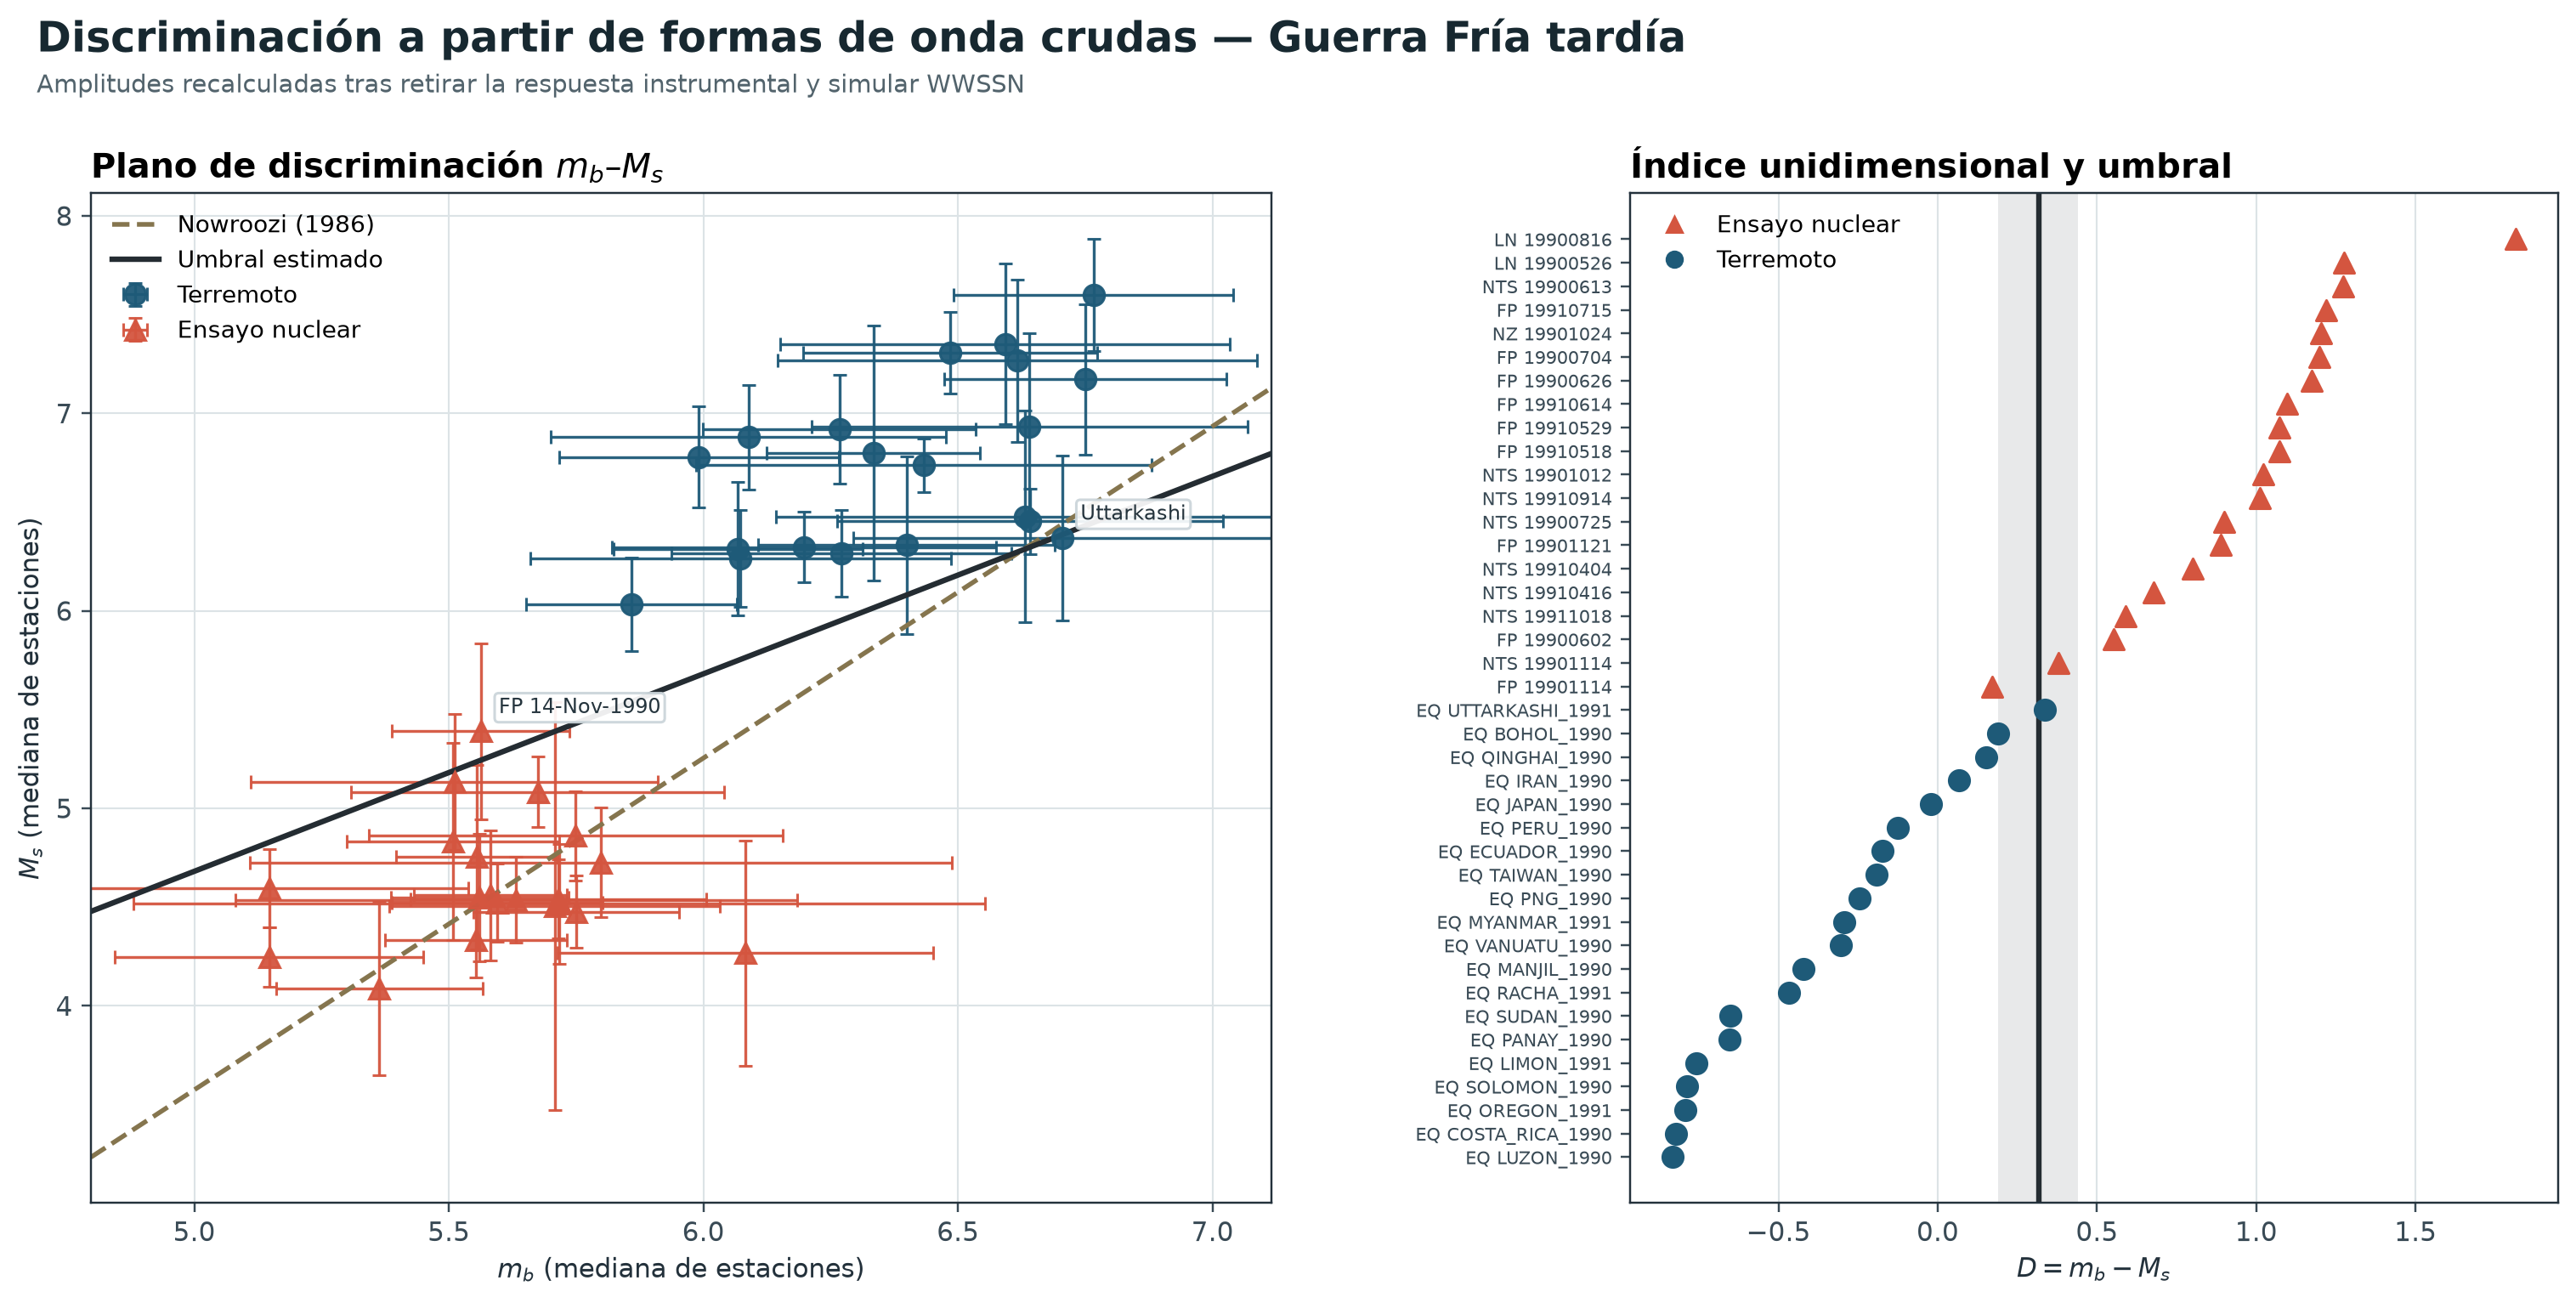
\includegraphics[width=0.95\textwidth]{discriminante_40}
   \caption{Plano $m_b$--$M_s$ y valores de $D$ de los 40 eventos del análisis reproducido. Línea continua: umbral $D=0.3185$; línea discontinua: frontera histórica de pendiente 1.68.}
   \label{fig:cohorte}
\end{figure}

\begin{figure}[H]
   \centering
   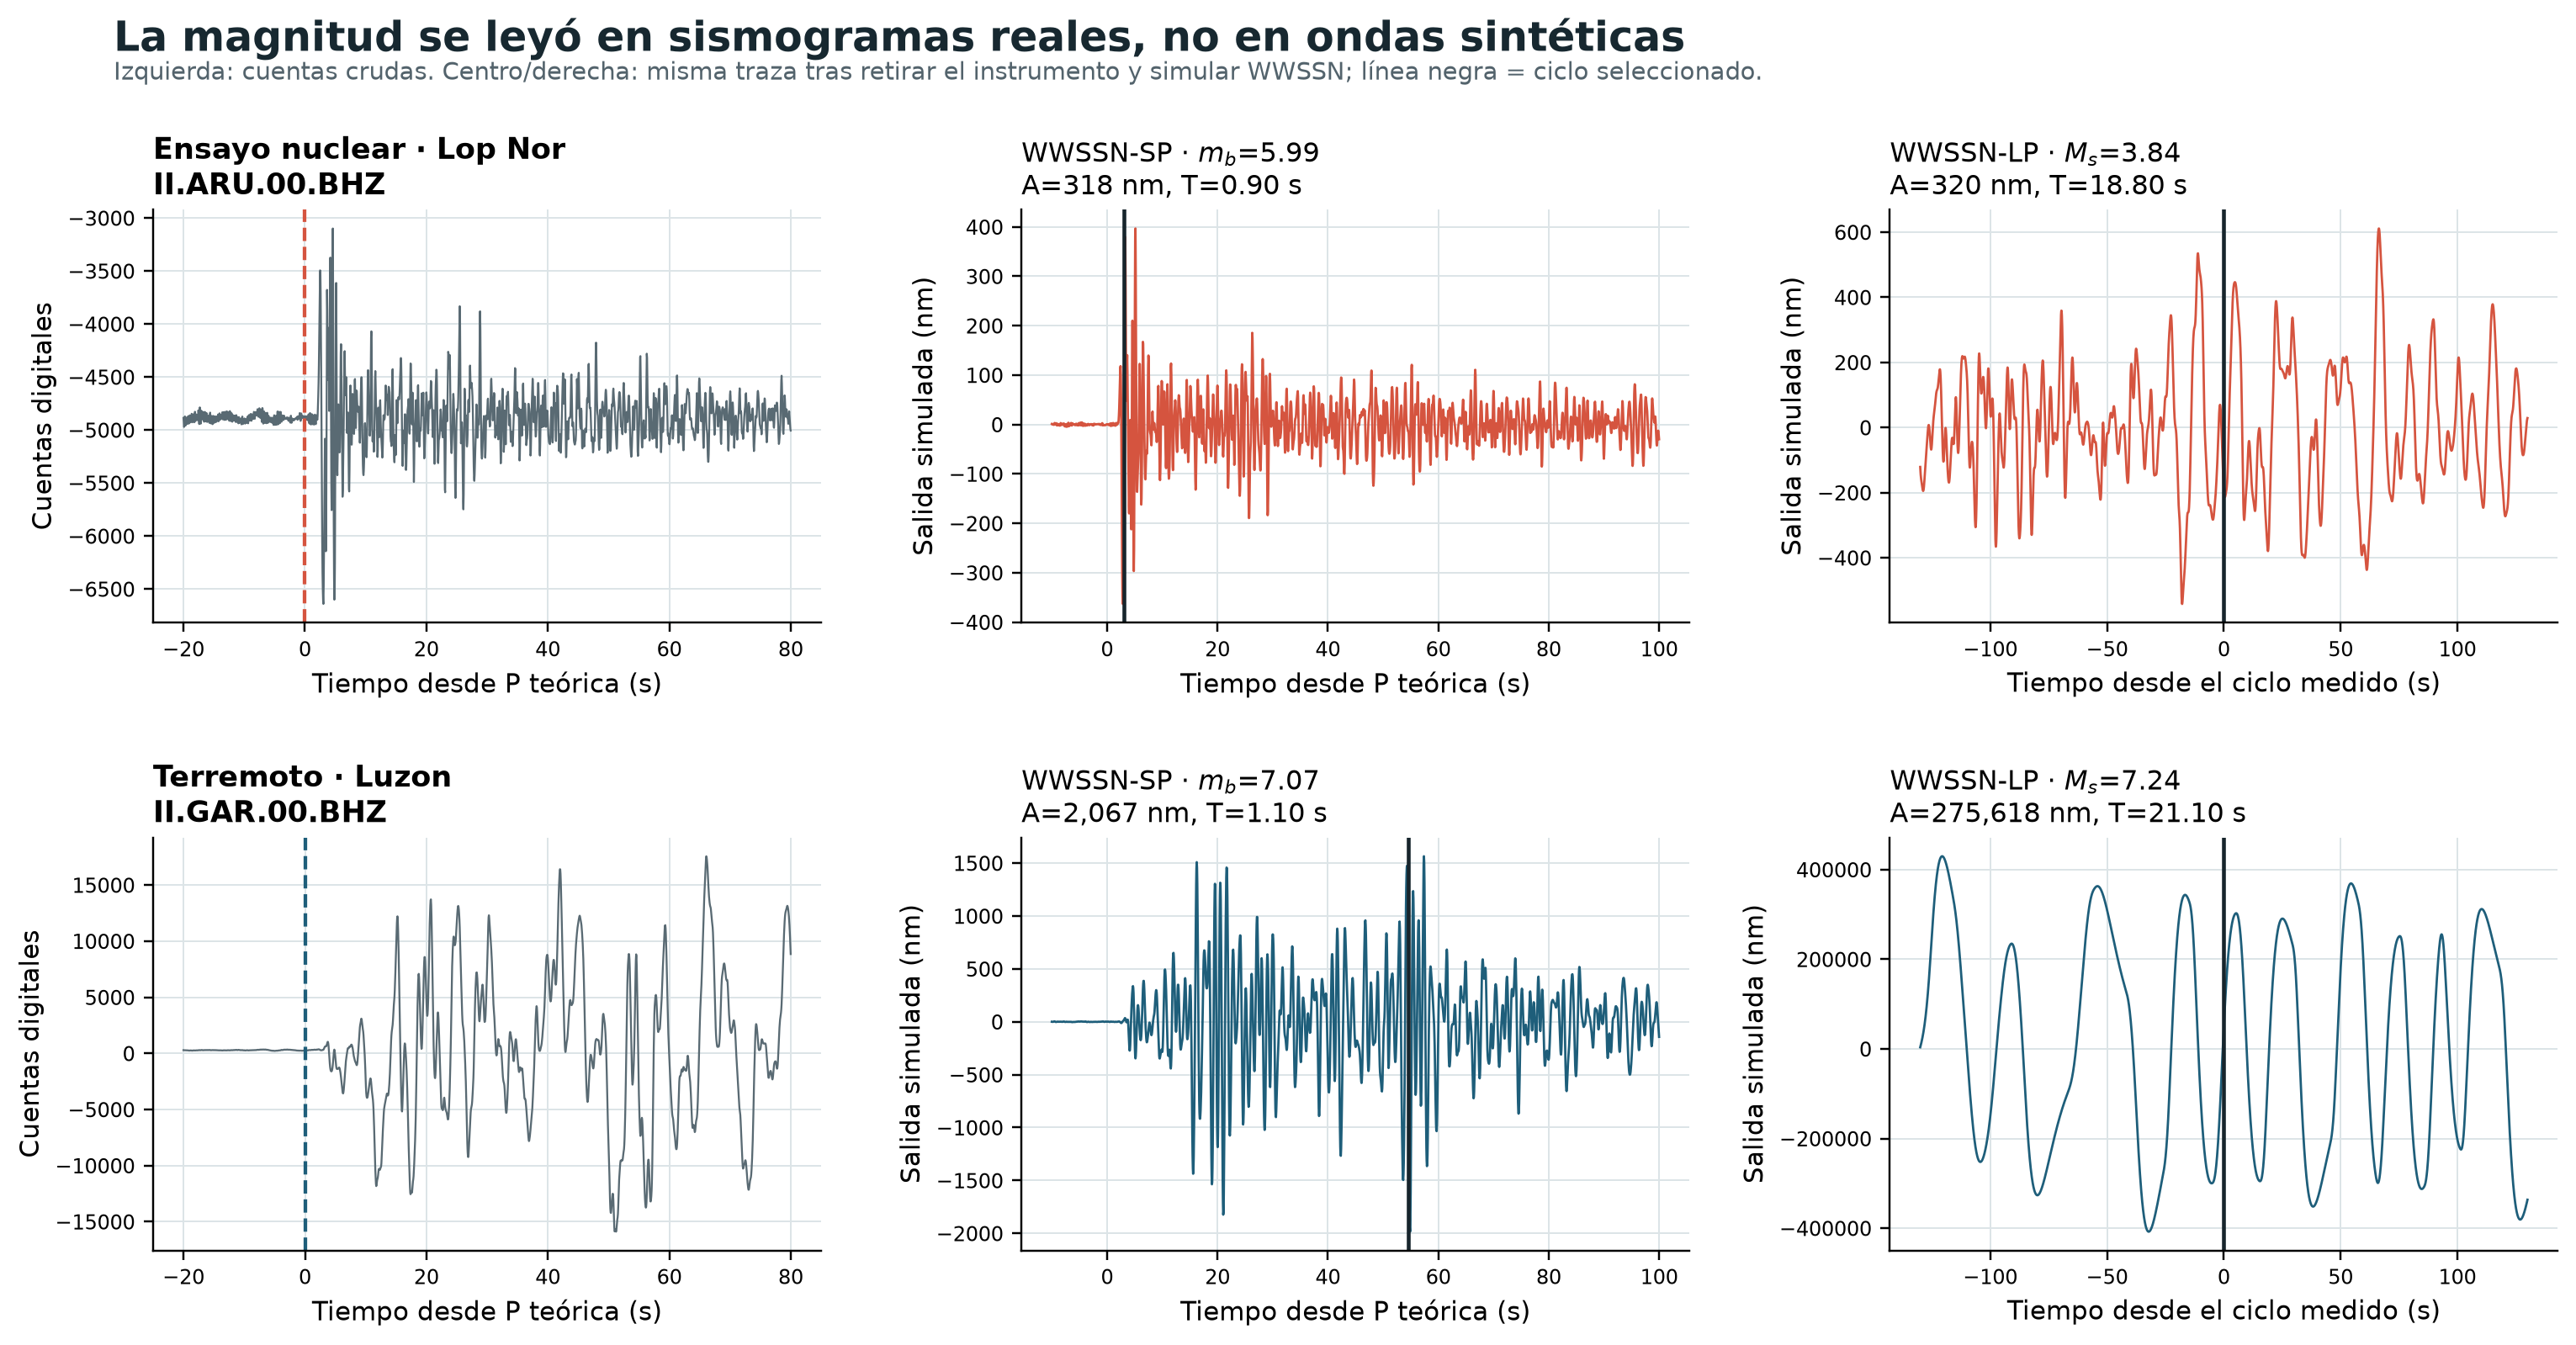
\includegraphics[width=0.95\textwidth]{trazas_reales}
   \caption{Registro crudo (izquierda) y simulaciones WWSSN-SP (centro) y WWSSN-LP (derecha) para una explosión en Lop~Nor y un sismo en Luzón. La línea negra marca el ciclo medido.}
   \label{fig:trazas}
\end{figure}

\subsection*{Sesgo de tamaño en la cohorte}
Los intervalos de $M_s$ de ambas clases no se traslapan (explosiones 4.09--5.39; sismos 6.03--7.60), y los de $m_b$ apenas lo hacen (Tabla~\ref{tab:sesgo}). Con el mismo procedimiento de validación, $M_s$ sola acierta 40/40 y un corte simple $m_b\geq5.85$ acierta 39/40, igual o mejor que $D$. Por lo tanto, el 95\% de aciertos no demuestra el efecto físico: la cohorte compara sismos grandes con explosiones pequeñas.

\begin{table}[H]
    \begin{center}
	    \begin{tabular}{|l|c|c|}
	    	\hline
	        Predictor & Un evento fuera & Una región fuera \\
	        \hline \hline
	        $D=m_b-M_s$ & 38/40 & 37/40 \\
	        \hline
	        $m_b$ solo & 37/40 & 36/40 \\
	        \hline
	        $M_s$ solo & 40/40 & 40/40 \\
	        \hline
        \end{tabular}
    \end{center}
	\caption{Aciertos en validación cruzada según el predictor usado en la regresión logística.}
	\label{tab:sesgo}
\end{table}

\subsection*{Calidad de las lecturas}
La simulación de ruido puro mostró que en ventanas de $m_b$ típicas ($\sim$150~s) el ruido solo alcanza $\text{SNR}\approx3$ en mediana y supera $\text{SNR}\geq2$ el 100\% de las veces; el 42\% de las lecturas $m_b$ de explosiones tiene $\text{SNR}<4$. Para $M_s$ el umbral es eficaz (el ruido supera $\text{SNR}\geq2$ solo en 1--5\% de los casos), aunque la $M_s$ de las explosiones es débil (SNR mediano 2.8). En los sismos, 17\% de los picos de $M_s$ cae en el último 5\% de la ventana, lo que indica que la ventana que termina en 3.0~km/s trunca la onda Rayleigh y subestima $M_s$. Esto afecta, por ejemplo, a Uttarkashi 1991, uno de los errores de clasificación. Los otros dos errores (Polinesia Francesa y Nevada, ambos del 14-nov-1990) ocurrieron con 65~min de diferencia, y el ruido previo al evento de Nevada está contaminado en 14 de 23 estaciones.

\subsection*{Par de igual $m_b$ dentro de la cohorte: Lop~Nor contra Taiwán}
La explosión de Lop~Nor del 16-ago-1990 y el sismo de Taiwán del 13-dic-1990 tienen $m_b=6.082$ y $6.073$. Sus $M_s$ son 4.27 y 6.27, de modo que $D=+1.81$ y $-0.19$ (Fig.~\ref{fig:par1}). En las 8 estaciones comunes, $D$ de la explosión es mayor en 8/8, con diferencia mediana de $+1.79$ e intervalo bootstrap al 95\% de $[1.34,\,2.52]$. El periodo típico de la onda P es 0.8~s en la explosión y 1.5~s en el sismo, lo que concuerda con la mayor frecuencia de esquina de la fuente explosiva.

\begin{figure}[H]
   \centering
   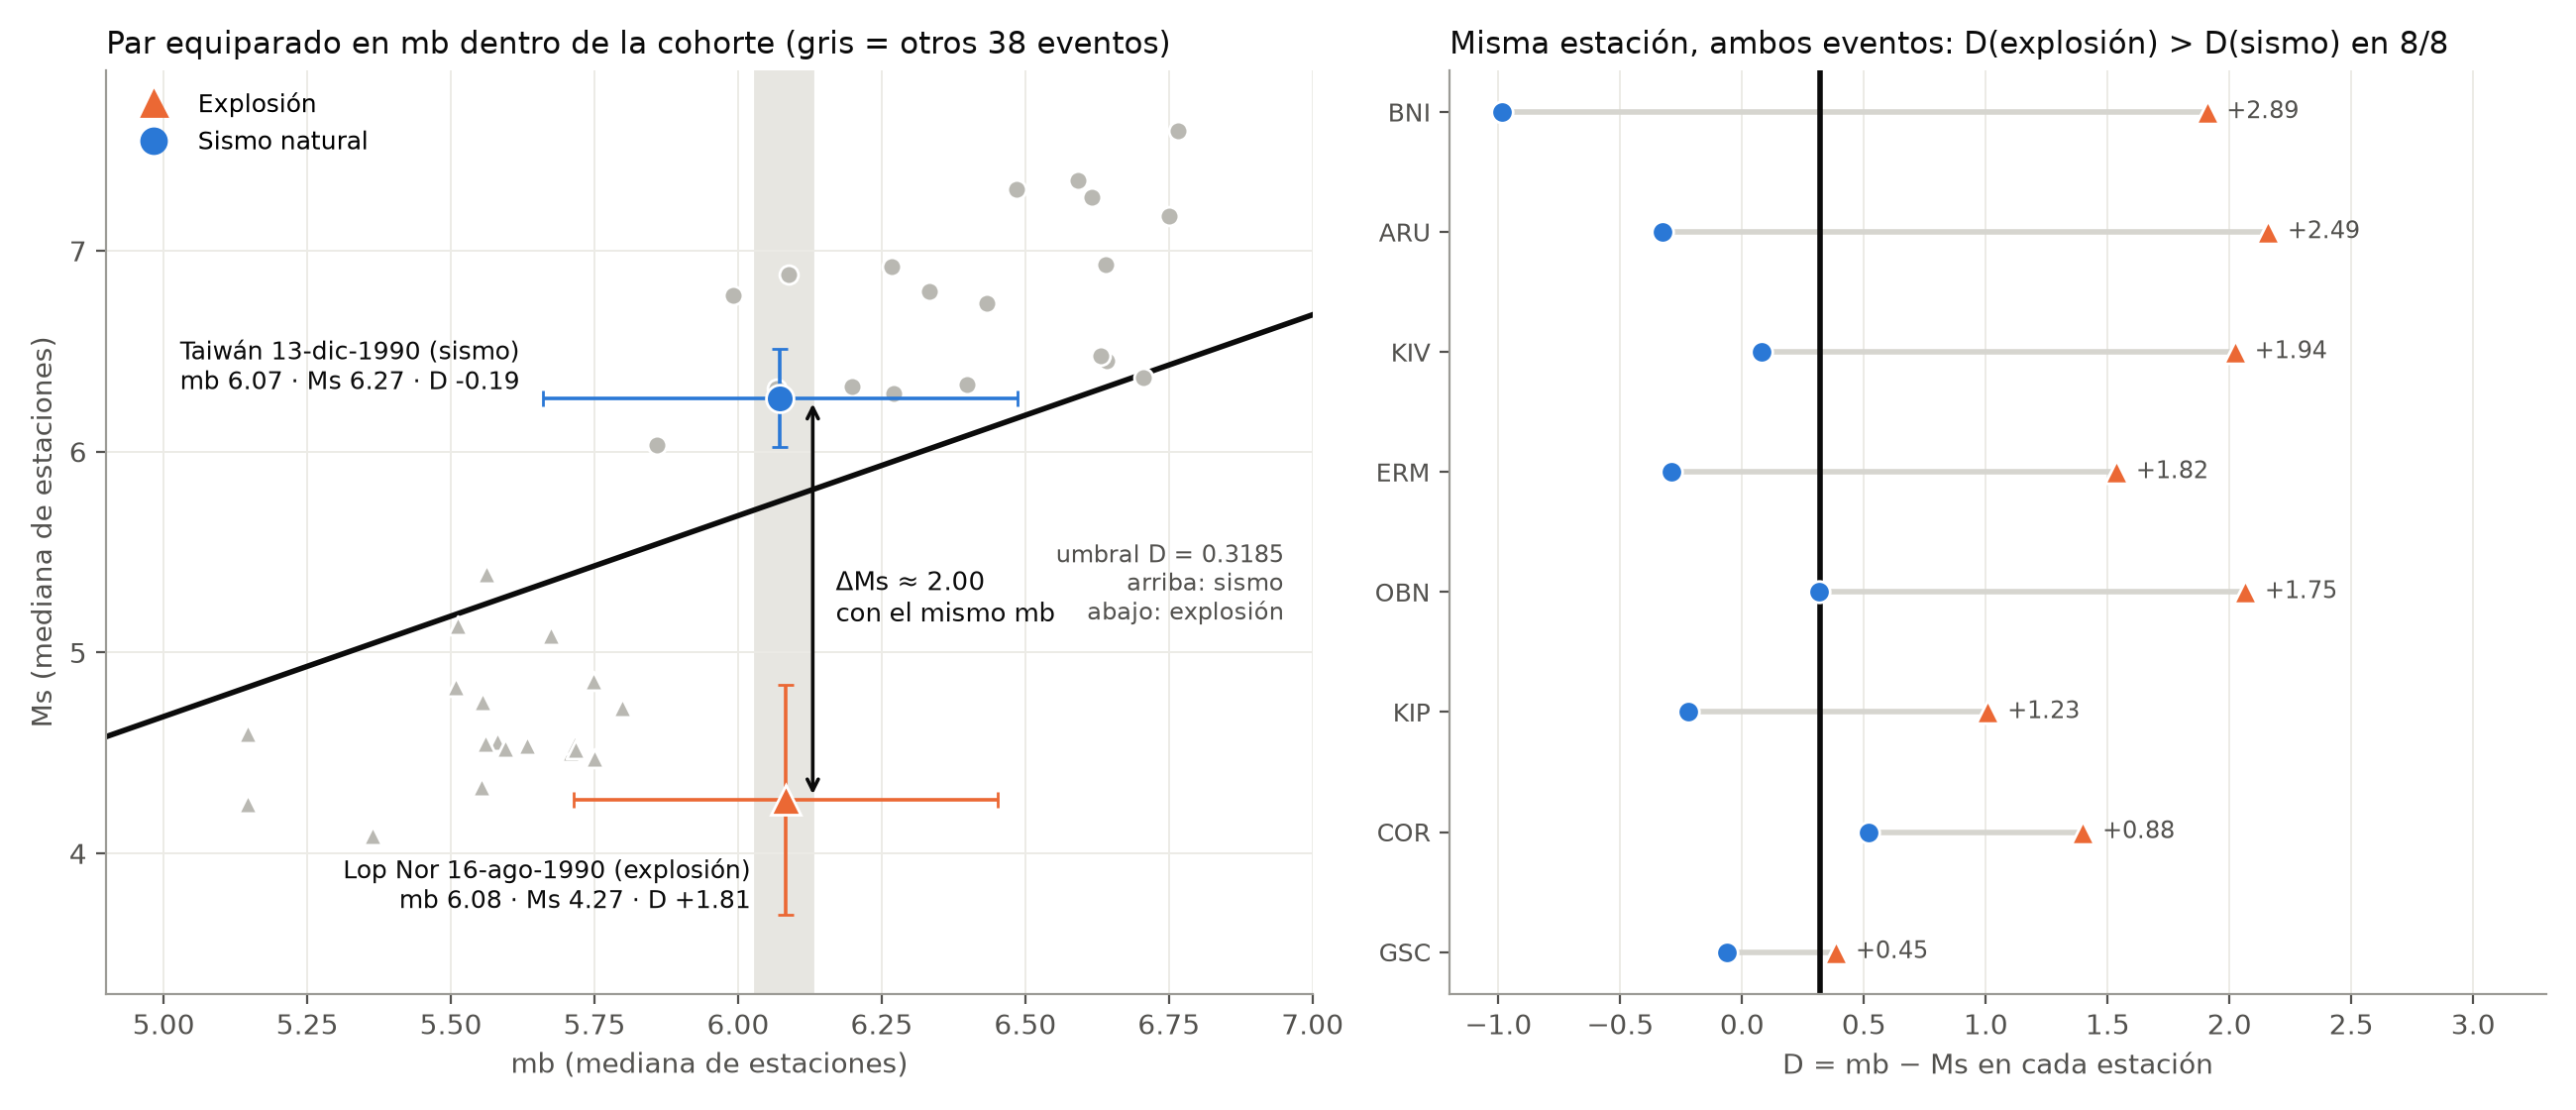
\includegraphics[width=0.95\textwidth]{par_lopnor_taiwan}
   \caption{Izquierda: ubicación del par Lop~Nor--Taiwán en el plano $m_b$--$M_s$. Derecha: $D$ medido en cada una de las 8 estaciones que registraron ambos eventos.}
   \label{fig:par1}
\end{figure}

\subsection*{Par nuevo: Corea del Norte 2016 contra Gyeongju 2016}
Con el código original, sin cambios, se descargaron 52 y 53 estaciones de las redes globales II/IU. Los resultados se resumen en la Tabla~\ref{tab:corea} y la Fig.~\ref{fig:par2}. Como referencia externa, no usada en el cálculo, el USGS reporta $m_b=5.3$ para la explosión y $M_w=5.4$ para el sismo.

\begin{table}[H]
    \begin{center}
	    \begin{tabular}{|l|c|c|}
	    	\hline
	        & Corea del Norte (explosión) & Gyeongju (sismo, 13 km) \\
	        \hline \hline
	        Fecha (UTC) & 2016-09-09 00:30:01 & 2016-09-12 11:32:55 \\
	        \hline
	        $m_b$ (lecturas) & $5.44\pm0.42$ (43) & $5.52\pm0.52$ (41) \\
	        \hline
	        $M_s$ (lecturas) & $4.27\pm0.69$ (24) & $5.17\pm0.34$ (52) \\
	        \hline
	        $D=m_b-M_s$ & $+1.17$ & $+0.35$ \\
	        \hline
	        $D$ con SNR$\geq3$ & $+0.99$ & $+0.25$ \\
	        \hline
	        Periodo típico de P & 0.8 s & 1.2 s \\
	        \hline
	        $P(\text{explosión})$, ec.~(\ref{eq:logit}) & 0.91 & 0.52 \\
	        \hline
	        Posición por $D$ entre 42 eventos & 8 & 21 \\
	        \hline
        \end{tabular}
    \end{center}
	\caption{Magnitudes calculadas para el par nuevo. Incertidumbre: $1.4826\times$MAD entre estaciones.}
	\label{tab:corea}
\end{table}

\begin{figure}[H]
   \centering
   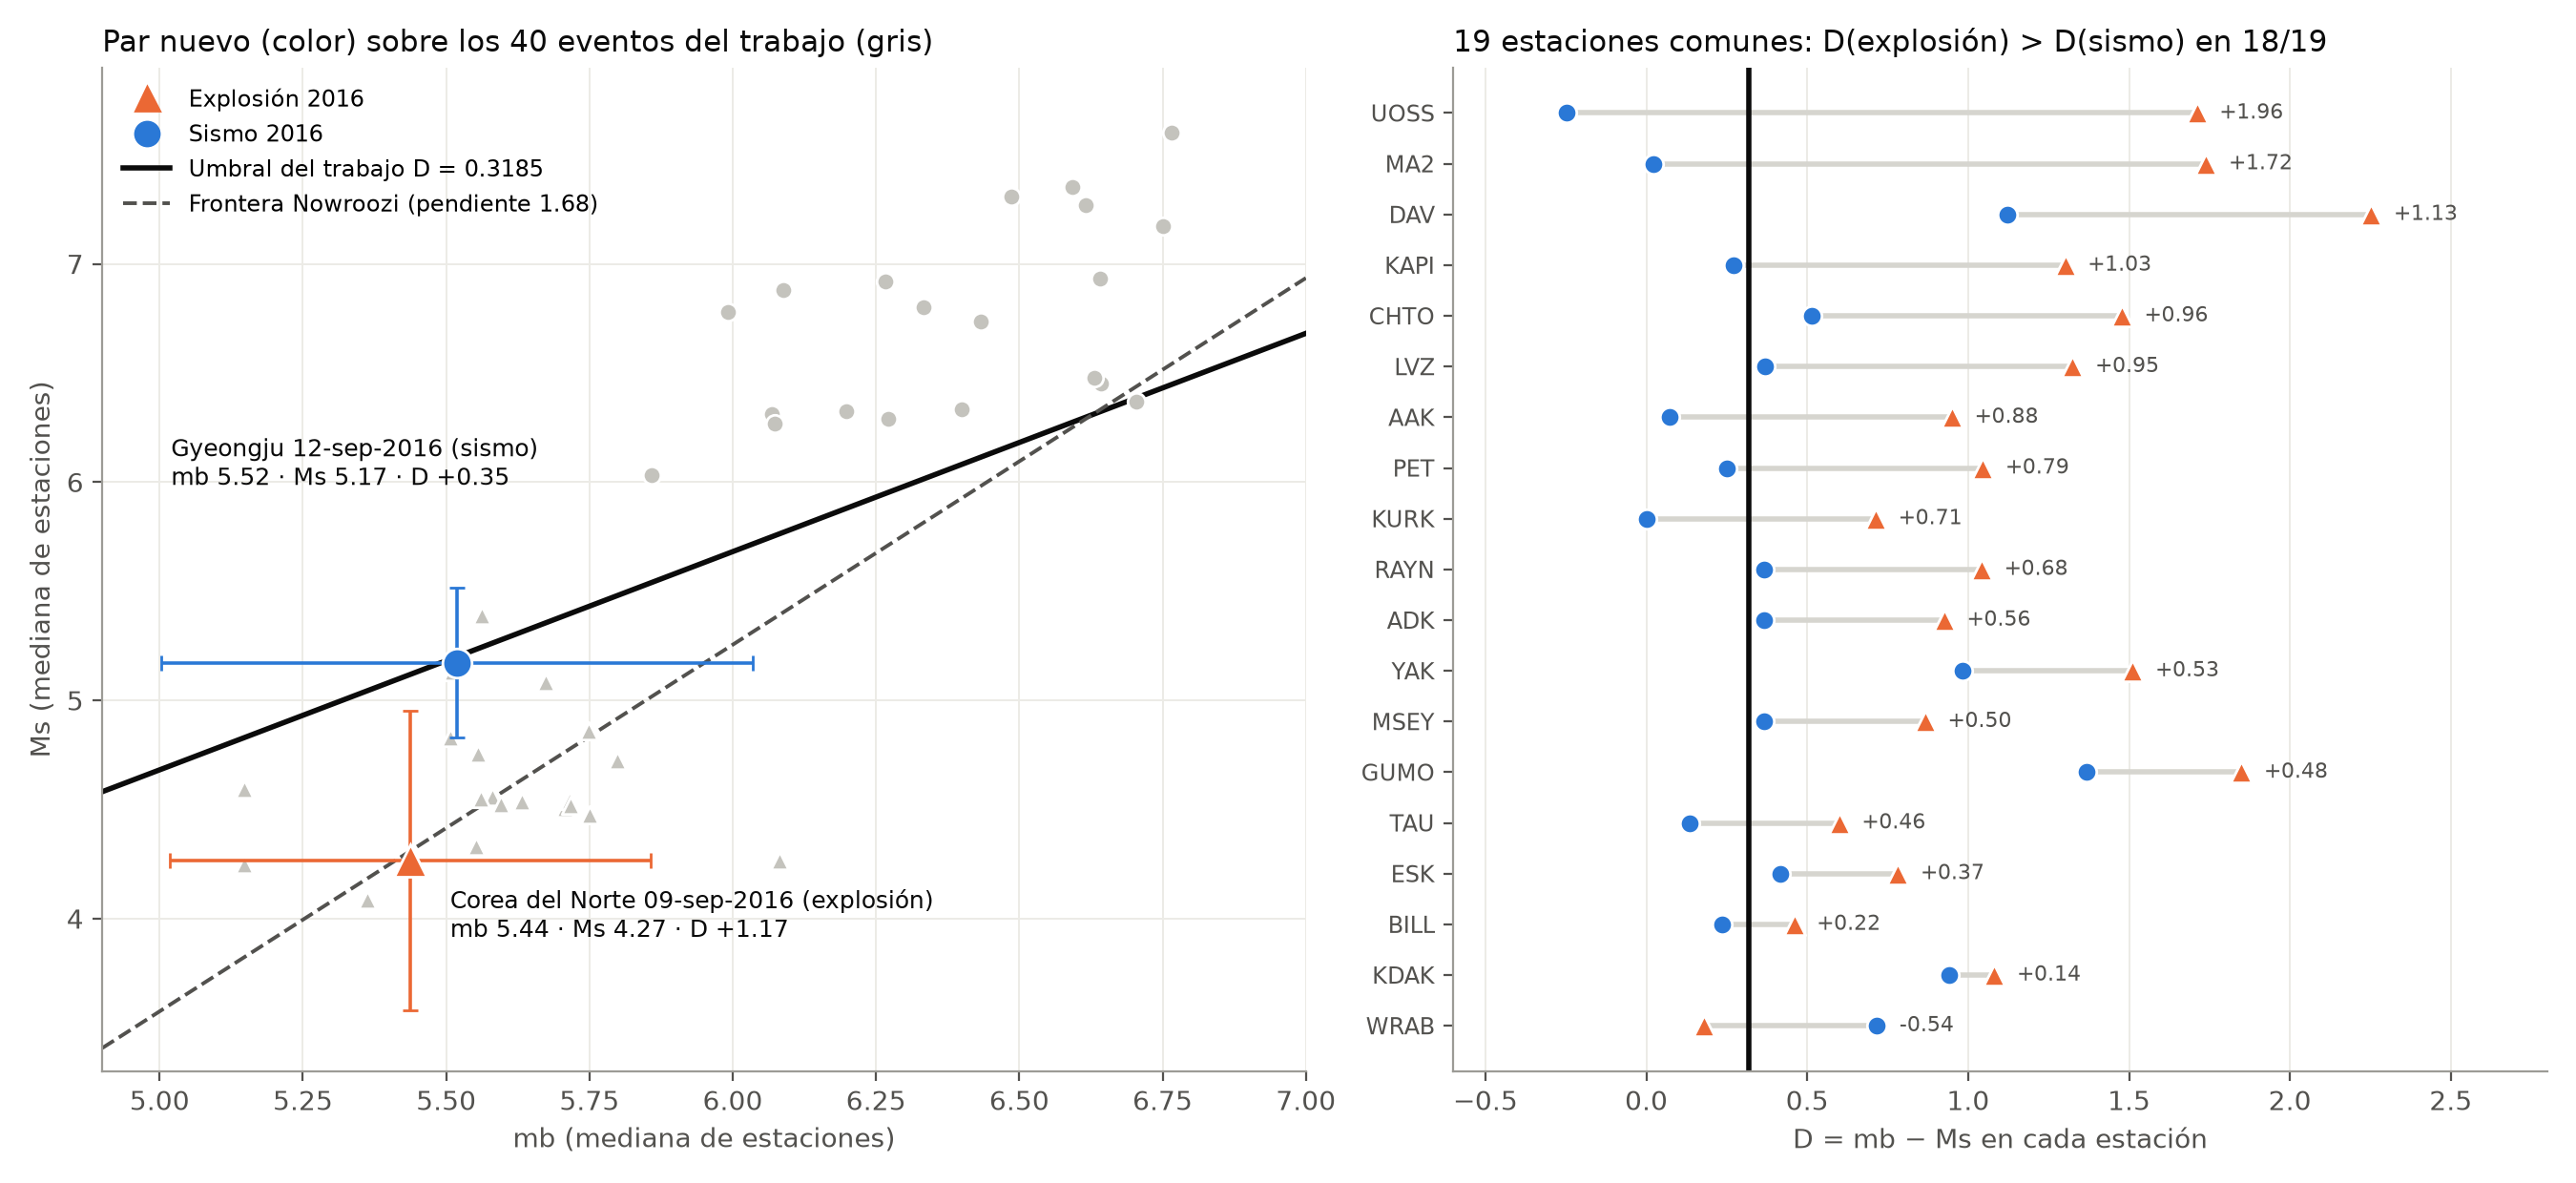
\includegraphics[width=0.95\textwidth]{par_corea_2016}
   \caption{Izquierda: par coreano de 2016 (color) sobre los 40 eventos (gris). Derecha: $D$ en las 19 estaciones comunes.}
   \label{fig:par2}
\end{figure}

A igual $m_b$ (diferencia de 0.08), la explosión tiene $M_s$ menor por 0.77 unidades, unas 6 veces menos amplitud de onda Rayleigh. En las 19 estaciones comunes, $D$ de la explosión es mayor en 18 casos; la diferencia mediana es $+0.68$, con intervalo al 95\% de $[0.26,\,1.17]$. Sin embargo, el sismo de Gyeongju queda en $D=0.346$, apenas por encima del umbral 0.3185, y la ec.~(\ref{eq:logit}) lo clasifica como explosión ($P=0.52$). La frontera inclinada de pendiente 1.68 (línea discontinua en la Fig.~\ref{fig:par2}) clasifica correctamente ambos eventos.

\section*{Conclusiones}

\begin{enumerate}
  \item El principio físico del discriminante $m_b$--$M_s$ se confirma \cite{stevens}. En dos pares independientes de igual $m_b$, uno de 1990 y otro de 2016 procesado desde cero, la explosión presenta $M_s$ menor, $D$ mayor en casi todas las estaciones comunes y ondas P de periodo más corto.
  \item El procesamiento (corrección instrumental, simulación WWSSN y fórmulas IASPEI) está correctamente implementado y es trazable: todas las cifras del análisis reproducido se recalcularon exactamente.
  \item El resultado cuantitativo del análisis original (umbral $D\geq0.3185$ con 95\% de aciertos) no demuestra por sí mismo el poder del discriminante, porque la cohorte está separada por tamaño y $M_s$ sola la clasifica perfectamente.
  \item Un umbral de $D$ constante no es transferible: el sismo de Gyeongju ($m_b\approx5.5$) cae del lado ``explosión''. En los sismos, $M_s$ no crece al mismo ritmo que $m_b$, por lo que la frontera debe tener pendiente mayor que 1, como las fronteras históricas.
  \item Como trabajo futuro se proponen: una cohorte con $m_b$ equiparado entre 4.5 y 6, un criterio de SNR que compare la señal con el máximo del ruido medido con el mismo estadístico, una ventana de $M_s$ extendida hasta $\sim$2.5~km/s, el tratamiento de no detecciones como cotas superiores y una comparación ciega con boletines internacionales.
\end{enumerate}

\begin{thebibliography}{99}

\bibitem{bowers} \fontsize{0.35cm}{0.5cm}\selectfont{D. Bowers y N. D. Selby, ``Forensic seismology and the Comprehensive Nuclear-Test-Ban Treaty'', \emph{Annual Review of Earth and Planetary Sciences}, Vol. 37, p. 209-236, 2009.}

\bibitem{stevens} \fontsize{0.35cm}{0.5cm}\selectfont{J. L. Stevens y S. M. Day, ``The physical basis of $m_b$:$M_s$ and variable frequency magnitude methods for earthquake/explosion discrimination'', \emph{Journal of Geophysical Research}, Vol. 90, No. B4, p. 3009-3020, 1985.}

\bibitem{iaspei} \fontsize{0.35cm}{0.5cm}\selectfont{P. Bormann y J. W. Dewey, ``The new IASPEI standards for determining magnitudes from digital data and their relation to classical magnitudes'', \emph{New Manual of Seismological Observatory Practice 2 (NMSOP-2)}, Information Sheet IS 3.3, GFZ Potsdam, 2014.}

\bibitem{gutenberg} \fontsize{0.35cm}{0.5cm}\selectfont{B. Gutenberg y C. F. Richter, ``Magnitude and energy of earthquakes'', \emph{Annali di Geofisica}, Vol. 9, p. 1-15, 1956.}

\bibitem{vanek} \fontsize{0.35cm}{0.5cm}\selectfont{J. Vaněk, A. Zátopek, V. Kárník \emph{et al.}, ``Standardization of magnitude scales'', \emph{Izvestiya Akademii Nauk SSSR, Seriya Geofizicheskaya}, No. 2, p. 108-111, 1962.}

\bibitem{iasp91} \fontsize{0.35cm}{0.5cm}\selectfont{B. L. N. Kennett y E. R. Engdahl, ``Traveltimes for global earthquake location and phase identification'', \emph{Geophysical Journal International}, Vol. 105, No. 2, p. 429-465, 1991.}

\bibitem{obspy} \fontsize{0.35cm}{0.5cm}\selectfont{M. Beyreuther, R. Barsch, L. Krischer \emph{et al.}, ``ObsPy: A Python toolbox for seismology'', \emph{Seismological Research Letters}, Vol. 81, No. 3, p. 530-533, 2010.}

\bibitem{sklearn} \fontsize{0.35cm}{0.5cm}\selectfont{F. Pedregosa \emph{et al.}, ``Scikit-learn: Machine learning in Python'', \emph{Journal of Machine Learning Research}, Vol. 12, p. 2825-2830, 2011.}

\bibitem{peterson} \fontsize{0.35cm}{0.5cm}\selectfont{J. Peterson, ``Observations and modeling of seismic background noise'', \emph{U.S. Geological Survey Open-File Report} 93-322, 1993.}

  \end{thebibliography}

\end{document}
